\documentclass{article}
\usepackage{amssymb}
\usepackage{amsmath}
\usepackage{algorithm} % Boxes/formatting around algorithms
\usepackage[noend]{algpseudocode} % Algorithms
\usepackage[normalem]{ulem}
\usepackage[margin=2cm]{geometry}
\usepackage[T1]{fontenc}
\usepackage[makeroom]{cancel}
\usepackage[pdftex]{graphicx}
\usepackage[final]{pdfpages}


\newcommand\lgh{\fontsize{17}{21}\usefont{T1}{cmdh}{m}{n}}
\newcommand\myrule{\par\noindent\rule{\textwidth}{4pt}\par}


\begin{document}

\myrule\medskip
\noindent{\lgh CS168 | Fall 2016 \hfill Introduction to Internet: Architecture \& Protocols\\[0.5ex]
Project 3: Measurement}\hfill{\scshape Peter B. Lee | October 2016}
\myrule
\section{Round Trip Time}
\begin{enumerate}
    \item
    Experiment A:
    \begin{enumerate}
        \item
        22\% never respond to pings. 35\% fail at least one ping. 
        \item CDF on next page.
        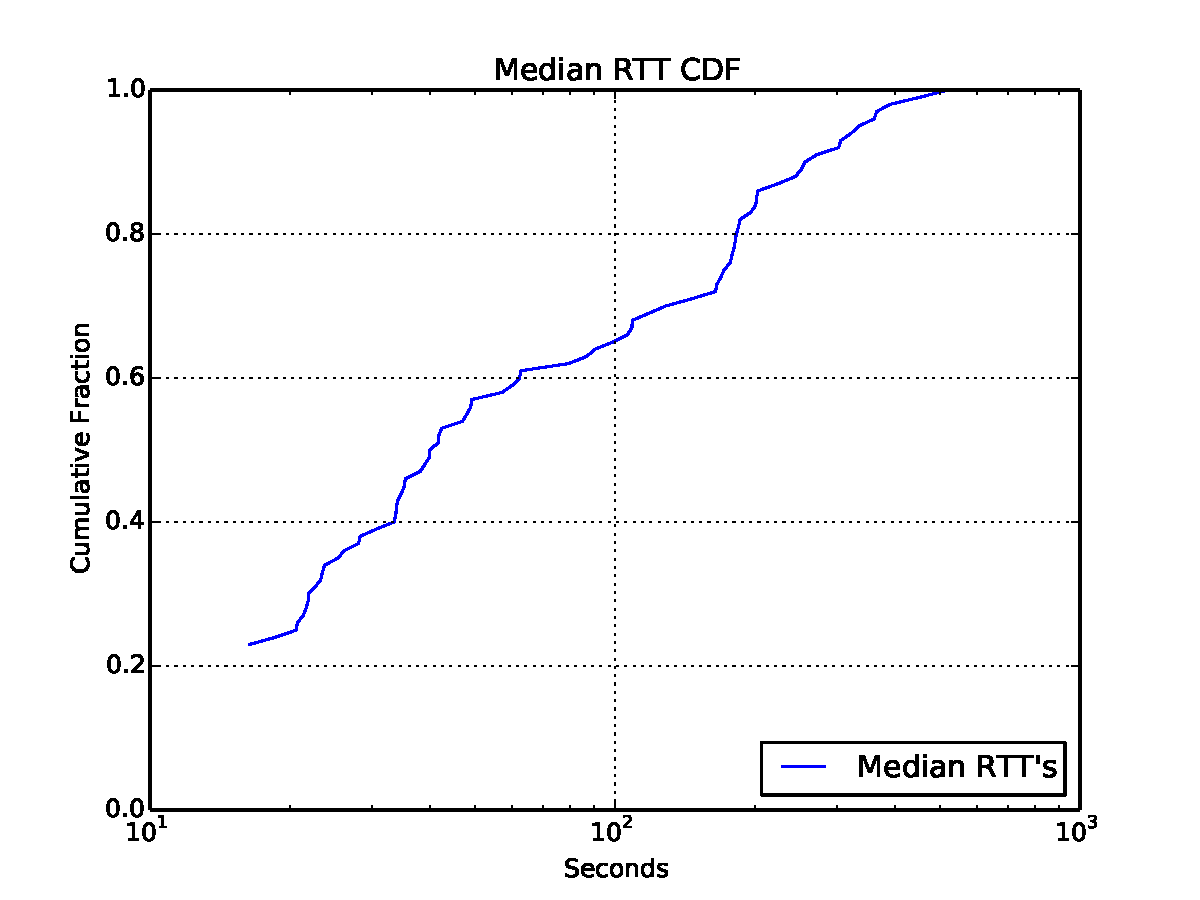
\includepdf[pages=1,pagecommand={}]{rtt_a_agg_ping_results.pdf}
    \end{enumerate}
    \item
    Experiment B:
    \begin{enumerate}
        \item
        For "google.com", median RTT: 95.495 ms, maximum RTT: 6.872 ms.\\
        It's loss rate is 0.0.\\
        For "todayhumor.co.kr", median RTT: 154.546 ms, maximum RTT: 11.985 ms.\\
        It's loss rate is 0.0.\\
        For "zanvarsity.ac.tz", median RTT: 680.526 ms, maximum RTT: 76.276 ms.\\
        It's loss rate is 2.0.\\
        For "taobao.com", median RTT: 668.561 ms, maximum RTT: 74.398 ms. \\ 
        It's loss rate is 0.8.
        \item CDF on next page.
        \item
        \begin{enumerate}
            \item
            The multiplier for google.com is $3.18537033 * 10^{-10} s^{2}/m$. The multipler for zanvarsity.ac.tz is $2.26999039 * 10^{-9} s^{2}/m$.
            \item
            The reason why the ping time is not equal to the speed of light time is due to several factors, one example being distance that the packets have to travel back and forth, using cables and routers. Due to this, trying to ping a location that is farther away such as zanvaristy.ac.tz's servers compared to google.com's yields for a greater median RTT. This would mean that a website's "physical location" contributes to the amount of time it takes to ping the website.
        \end{enumerate}
    \end{enumerate}
    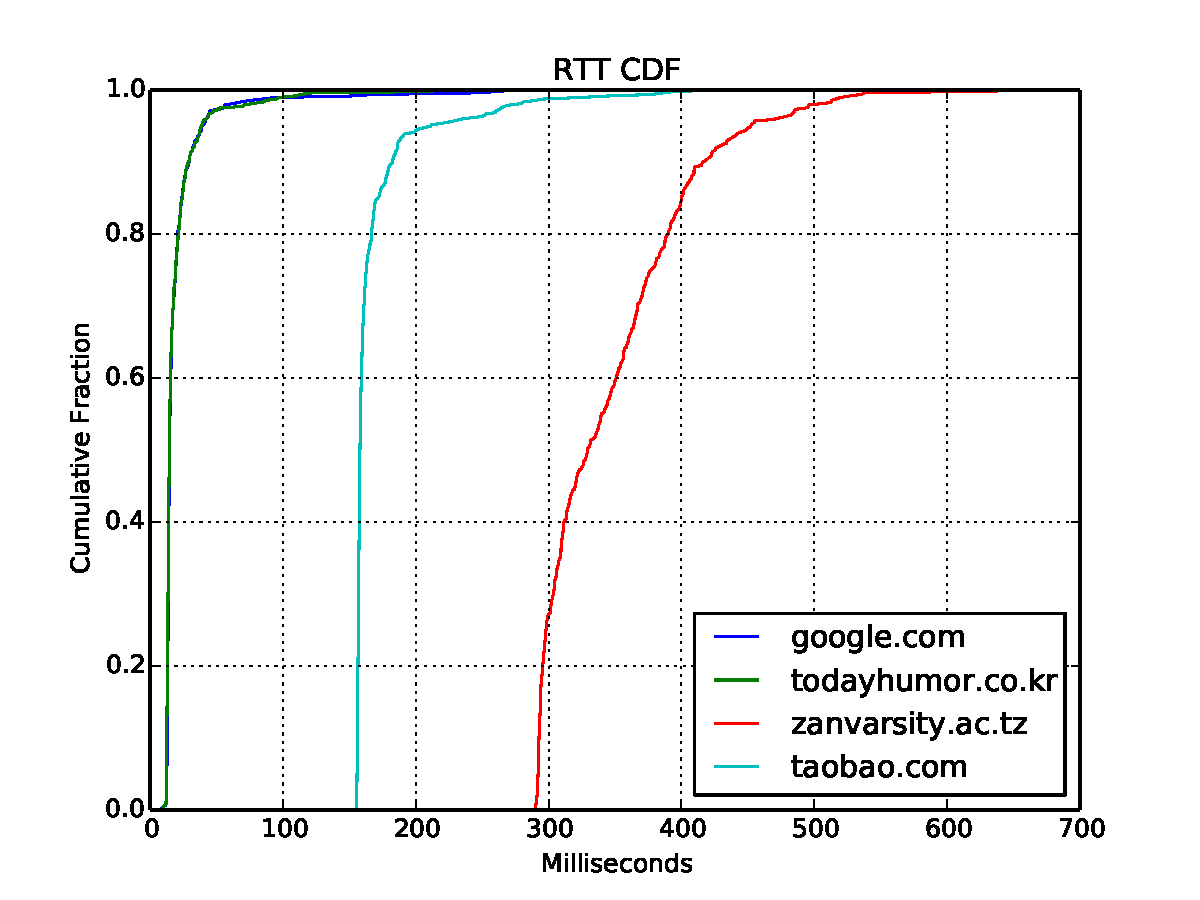
\includepdf[pages=1]{rtt_b_raw_results.pdf}
\end{enumerate}
\section{Routing}
\begin{enumerate}
    \item Experiment A
    \begin{enumerate}
        \item Which ASes are Berkeley directly connected to?
        \item Which traceroute traverses the most number of ASes? How about the least number of ASes?
        \item Which websites' routes are load-balanced?
        \item Are the observed routes stable over multiple runs? For each website, how many unique routes did you observe?
        \item Using one sentence, please explain one advantage of having stable routes.\\
            The ASes of Berkeley are directly connected to
    \end{enumerate}
    \item Experiment B
    \begin{enumerate}
    \item How many hops do you observe in each route when you run traceroute from your computer? How many hops do you observe in the reverse direction?\\ \\
    Number of hops from our computer to the public servers:\\
    18 hops to tpr-route-server.saix.net\\
    13 hops to route-server.ip-plus.net\\
    14 hops to route-views.oregon-ix.net\\
    13 hops to route-views.on.bb.telus.com\\
    Number of hops to our computer from the public servers:\\
    17 hops to tpr-route-server.saix.net\\
    23 hops to route-server.ip-plus.net\\
    9 hops to route-views.oregon-ix.net\\
    14 hops to route-views.on.bb.telus.com
    \item Are these routes symmetric? How many are symmetric and how many are not?\\
    None of these routes are symmetric.
    \item What might cause asymmetric routes? List one or two reasons? \\
    Traffic congestion is one potential cause of routing asymmetry.
    \end{enumerate}
\end{enumerate}
\section{Naming}

\end{document}
